\section{Probabilidade condicional e independência}

De que forma devemos calcular a probabilidade de eventos sabendo
que um certo evento ocorreu?

\begin{figure}[ht!]
    \centering
    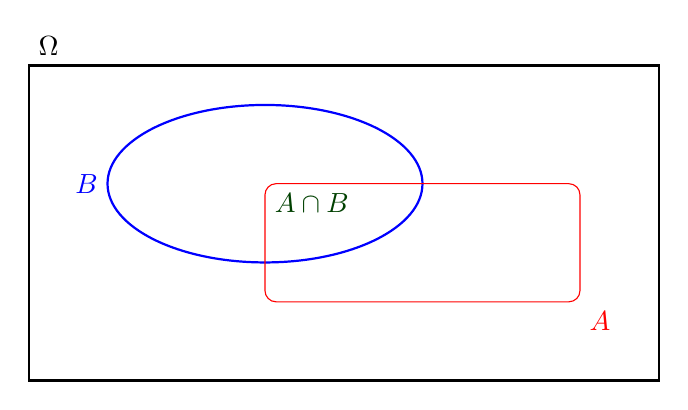
\begin{tikzpicture}
        \draw[thick] (-4, -2) rectangle (4, 2);
        \node[anchor=south west] at (-4, 2) {$\Omega$};

        \draw[thick, blue] (-1, 0.5) ellipse[x radius=2, y radius=1];
        \node[anchor=east, blue] at (-3, 0.5) {$B$};

        \draw[rounded corners, red] (-1, 0.5) rectangle (3, -1);
        \node[anchor=north west, red] at (3, -1) {$A$};

        \node[anchor=north west, green!25!black] at (-1, 0.5) {$A \cap B$};
    \end{tikzpicture}
    \caption{Situação oiginal}
    \label{fig:ch01-condicional-antes}
\end{figure}

\begin{obs}
    Lembe-se que $\Omega$ é outra notação para o espaço amostral.
\end{obs}

\begin{figure}[ht!]
    \centering
    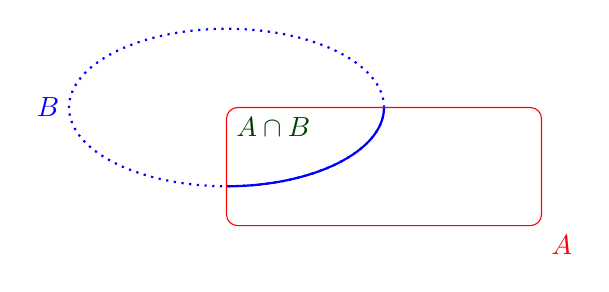
\begin{tikzpicture}
        \draw[thick, blue, dotted] (-1, 0.5) ellipse[x radius=2, y radius=1];
        \node[anchor=east, blue] at (-3, 0.5) {$B$};

        \draw[thick, blue] (-1, -.5) arc (-90:0:2 and 1);
        
        \draw[rounded corners, red] (-1, 0.5) rectangle (3, -1);
        \node[anchor=north west, red] at (3, -1) {$A$};

        \node[anchor=north west, green!25!black] at (-1, 0.5) {$A \cap B$};
    \end{tikzpicture}
    \caption{Situação após a ocorrência do evento $A$}
    \label{fig:ch01-condicional-depois}
\end{figure}

\begin{definition}[Pobabilidade Condicional]
    $A$ e $B$ são eventos de um espaço amostral, em que $\Prob(A) > 0$.
    A probabilidade condicional de $B$ dado o evento $A$ é definida como
    \begin{align}
        \Prob(B | A) &= \frac{\Prob(B \cap A)}{\Prob(A)} 
            \label{eq:ch01-condicional}
    \end{align}

    \begin{obs}
        Se $\Prob(A) = 0$, não se define $\Prob(B | A)$.
    \end{obs}
\end{definition}

Dessa definição, obtemos a fórmula do produto:
\begin{align}
    \Prob(B \cap A) &= \Prob(B | A) \cdot \Prob(A)
        \label{eq:ch01-regra-produto}
\end{align}

\begin{example}
    Considere a situação ilustrada nas
    \cref{fig:ch01-condicional-antes,fig:ch01-condicional-depois}.
    Vamos analisar como a pobabilidade do evento $B$ se altera
    diante de novas informações.

    Inicialmente (\cref{fig:ch01-condicional-antes}), não há
    infomação sobre a ocorrência de outro evento. Podemos escrever:
    \begin{align*}
        \Prob(B) &= \Prob(B | \Omega) \\
        &= \frac{\Prob(B \cap \Omega)}{\Prob(\Omega)}
    \end{align*}
    lembrando que $B \cap \Omega = B$ e $\Prob(\Omega) = 1$ (pelo axioma
    \labelcref{it:ch01-axioma-3} na \cref{def:axiomatica})
    
    Por outro lado, quando o evento $A$ ocorre
    (\cref{fig:ch01-condicional-depois}), temos
    \begin{align*}
        \Prob(B | A) &= \frac{\Prob(B \cap A)}{\Prob(A)} 
    \end{align*}

    Comparando as expressões acima, é possível observar
    que quando a ocorrência do evento $B$ é analisada
    dada a ocorrência do evento $A$, é como se o evento $A$
    tomasse as vezes como um novo espaço amostral.
\end{example}

\begin{lemma}
    A probabilidade condicional satisfaz a definição axiomática.
\end{lemma}

\begin{lemma}
    $A_1, A_2, \cdots, A_n$ são eventos de um espaço amostral,
    com $n \geq 2$. Temos:
    \begin{align}
        \Prob(A_1 \cap A_2 \cap \cdots \cap A_n) &=
            \Prob(A_1)
            \cdot \Prob(A_2 | A_1)
            \cdot \Prob(A_3 |A_2 \cap A_1) \notag \\
        &\phantom{=} \cdot \ldots
        \cdot \Prob(A_n | A_{n-1} \cap \cdots \cap A_2 \cap A_1)
    \end{align}
\end{lemma}

\begin{definition}[Independência de eventos]
    $A$ e $B$ são eventos de um espaço amostral, em que $\Prob(A) > 0$
    e $\Prob(B) > 0$. O evento $B$ é independente do evento $A$ se:
    \begin{align}
        \Prob(B | A) &= \Prob(B) \label{eq:ch01-independencia}
    \end{align}
\end{definition}

\begin{obs}
    Se $B$ é independente de $A$,
    então $A$ é independente de $B$.

    \begin{proof}
        Se $B$ é independente de $A$, então
        \begin{align*}
            \Prob(A \cap B) &= \Prob(A) \cdot \Prob(B)
        \end{align*}
        Calculamos
        \begin{align*}
            \Prob(A | B) &= \frac{\Prob(A \cap B)}{\Prob(B)}  \\
            &= \frac{\Prob(A) \cdot \cancel{\Prob(B)}}
                {\cancel{\Prob(B)}}
            = \Prob(A)
        \end{align*}
    \end{proof} 
\end{obs}

\begin{definition}
    Os eventos $A_1, A_2, \cdots, A_n\ (n \geq 2)$ de um espaço amostral
    são independentes se
    \begin{align*}
        \Prob(A_{i_1} \cap A_{i_2} \cap \cdots \cap A_{i_k})
        &= \Prob(A_{i_1}) \cdot \Prob(A_{i_2})
        \cdot \ldots \cdot \Prob(A_{i_k})
    \end{align*}
    para todo $k \in \{2, 3, \cdots, n\}$ e
    todo $\{i_1, i_2, \cdots, i_n\} \subset \{1, 2, \cdots, n\}$ tais que
    $i_1 < i_2 < \cdots < i_n$.
\end{definition}

\begin{example}
    Espaço amostral com $N = 4$ elementos.

    \begin{center}
        \centering
        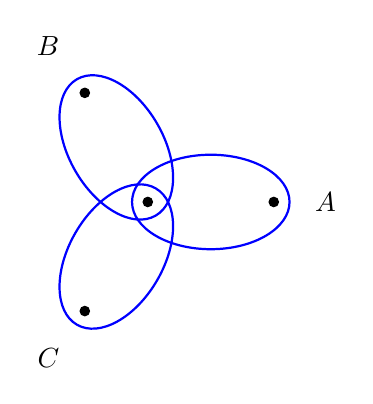
\begin{tikzpicture}[scale=0.2]
            \pgfmathsetmacro{\a}{5}
            \pgfmathsetmacro{\b}{4}
            \pgfmathsetmacro{\c}{3}
            \pgfmathsetmacro{\t}{\c/10}
            
            \draw[thick, blue] (\b, 0)
                ellipse[x radius=\a, y radius=\c];
            \node[anchor=west] at ({2*\a*cos(0)}, {2*\a*sin(0)}) {$A$};

            \draw[thick, blue] (\b, 0)
                ellipse[
                    x radius=\a,
                    y radius=\c,
                    rotate around={120:(-\b,0)}];
            \node[anchor=south east] at ({2*\a*cos(120)}, {2*\a*sin(120)}) {$B$};

            \draw[thick, blue] (\b, 0)
                ellipse[
                    x radius=\a,
                    y radius=\c,
                    rotate around={240:(-\b,0)}];
            \node[anchor=north east] at ({2*\a*cos(240)}, {2*\a*sin(240)}) {$C$};

            \filldraw (0, 0) circle (\t);
            \filldraw ({2*\b*cos(0)}, {2*\b*sin(0)}) circle (\t);
            \filldraw ({2*\b*cos(120)}, {2*\b*sin(120)}) circle (\t);
            \filldraw ({2*\b*cos(240)}, {2*\b*sin(240)}) circle (\t);
        \end{tikzpicture}
    \end{center}

    Calculamos
    \begin{align*}
        \Prob(A) &= \Prob(B) = \Prob(C) = \frac{2}{4} = \frac{1}{2}
    \end{align*}

    Em seguida, calculamos
    \begin{align*}
        \Prob(A \cap B) &= \frac{1}{4} = \Prob(A) \cdot \Prob(B) \\
        \Prob(A \cap C) &= \frac{1}{4} = \Prob(A) \cdot \Prob(C) \\
        \Prob(B \cap C) &= \frac{1}{4} = \Prob(B) \cdot \Prob(C) \\
        \Prob(A \cap B \cap C) &= \frac{1}{4} 
        \neq \Prob(A) \cdot \Prob(B) \cdot \Prob(C) = \frac{1}{8}
    \end{align*}

    Portanto, os três evendos são independentes aos pares,
    mas não são conjuntamente independentes.
\end{example}

\begin{example}[O dilema do pisioneiro]
    Três pisioneiros ($A$, $B$ e $C$) têm históricos semelhantes
    e solicitaram liberdade condicional. O juiz decidiu que vai liberar
    dois prisioneiros

    O prisioneiro $A$ é amigo do guarda do presídio. O prisioneiro
    $A$ considera pedir que o guarda revele um dos prisioneiros liberados
    e que não seja ele mesmo (caso $A$ seja um dos liberados).

    \bigskip
    Os eventos $E_A$, $E_B$ e $E_C$ representam a liberação dos prisioneiros.
    Analogamente, temos os eventos $E_{AB}$, $E_{AC}$ e $E_{BC}$

    Definimos $I_j$ o evento que representa a informação do guarda,
    sendo que $j \in \{B, C\}$, e $\Prob(I_B) = \Prob(I_C) = \frac{1}{2}$.

    Temos que calcular $\Prob(E_A)$, $\Prob(E_A | I_B)$ e $\Prob(E_A | I_C)$.

    \bigskip
    $E_A = E_{AB} \cup E_{AC}$, sendo que $E_{AB}$ e $E_{AC}$
    são mutuamente exclusivos.

    \begin{center}
        \begin{tabular}{cc}
            \toprule
            Evento & Pobabulidade \\
            \midrule
            $E_{AB} \cap I_B$ 
                & $\begin{array} {rl}
                    \Prob(E_{AB} \cap I_B) 
                    &= \Prob(I_B | E_{AB}) \cdot \Prob(E_{AB}) \\
                    &= 1 \cdot \sfrac{1}{3} = \sfrac{1}{3} 
                    \end{array}$ \\
            $E_{AC} \cap I_C$ 
                & $\begin{array} {rl}
                    \Prob(E_{AC} \cap I_C) 
                    &= \Prob(I_C | E_{AC}) \cdot \Prob(E_{AB}) \\
                    &= 1 \cdot \sfrac{1}{3} = \sfrac{1}{3}
                    \end{array}$ \\
            $E_{BC} \cap I_B$ 
                & $\begin{array} {rl}
                    \Prob(E_{BC} \cap I_B)
                    &= \Prob(I_B | E_{BC}) \cdot \Prob(E_{BC}) \\
                    &= \sfrac{1}{2} \cdot \sfrac{1}{3} = \sfrac{1}{6}
                    \end{array}$ \\
            $E_{BC} \cap I_C$ 
                & $\begin{array} {rl}
                    \Prob(E_{BC} \cap I_C) 
                    &= \Prob(I_C | E_{BC}) \cdot \Prob(E_{BC}) \\
                    &= \sfrac{1}{2} \cdot \sfrac{1}{3} = \sfrac{1}{6}
                    \end{array}$ \\
            \bottomrule
        \end{tabular}
    \end{center}

    Calculamos $\Prob(E_A | I_B)$:
    \begin{align*}
        \Prob(E_A | I_B) &= \frac{\Prob(E_A \cap I_B)}{\Prob(I_B)} \\
        &= \frac{\Prob((E_{AB} \cup E_{AC}) \cap I_B)}{\Prob(I_B)} \\
        &= \frac{\Prob((E_{AB} \cap I_B) \cup (E_{AC} \cap I_B)))}
            {\Prob(I_B)} \\
        &= \frac{\Prob(E_{AB} \cap I_B) + \Prob(E_{AC} \cap I_B)}
            {\Prob(I_B)} \\
        &= \frac{\sfrac{1}{3} + 0}
            {\sfrac{1}{2}} = \frac{2}{3}
    \end{align*}

    Analogamente, $\Prob(E_A | I_C) = \frac{2}{3}$.

    Se o guarda falar que $B$ será libertado, o prisioneiro $A$
    considerou os pares $AB$ e $BC$, com probabilidades iguais a $\frac{1}{2}$.
    Antes da informação do guarda, $\Prob(E_A) = \frac{2}{3}$.
\end{example}

\begin{example}[Problema do séc. \romanum{18}]
    O evento $A$ representa pelo menos um resultado "6"
    em quatro lançamentos de um dado.

    O evento $B$ representa pelo menos um resultado "6,6"
    em 24 lançamentos de dois dados.

    \bigskip
    Calculamos
    \begin{align*}
        \Prob(A) &= \frac{1}{6} \cdot 4 = \frac{2}{3}
    \end{align*}
    e
    \begin{align*}
        \Prob(B) &= \frac{1}{36} \cdot 24 = \frac{2}{3}
    \end{align*}
    
    Ou seja, $\Prob(A) = \Prob(B)$.

    \bigskip
    Calculamos
    \begin{align*}
        \Prob(\stcomp{A}) &= \left(\frac{5}{6}\right)^4 
        = 0.4823
    \end{align*}
    e
    \begin{align*}
        \Prob(\stcomp{B}) &= \left(\frac{35}{36}\right)^{24}
        = 0.5086
    \end{align*}
    supondo independência.

    \begin{obs}
        Note que os resultados são incoerentes, mostrando que algo não
        foi considerado nesta solução.
    \end{obs}
\end{example}